% !TEX encoding = UTF-8
% !TEX TS-program = pdflatex
% !TEX root = ../tesi.tex

\chapter{Introduction}
	\section{Radio Propagation Models}
		A \gls{rpma} is an empirical mathematical formulation used to model the propagation of radio waves as a function of frequency, distance, transmission power and other variables. Over the years various RPMs have been developed, some aiming at modelling a general situation, and others more useful in specific scenarios. For example, implementations range from the more general free space model, where only distance and power are considered, to more complex models which account for shadowing, reflection, scattering, and other multipath losses. Moreover, it is important to keep into consideration the computational complexity and scalability of the model: some have poor accuracy but are scalable, while others have very good accuracy but can only work for small sets of nodes. As always, it is very important to find the right tradeoff between complexity and accuracy.
		
		
		The authors of \cite{6298165} classify the propagation models offered by the network simulator ns-3 in three different categories:
		\begin{itemize}
			\item \textbf{Abstract} propagation loss models, for example the Maximal Range model (also known as Unit Disk), which establishes that all transmissions within a certain range are received without any loss;
			\item \textbf{Deterministic} path loss models, such as the Friis propagation model, which models quadratic path loss as it occurs in free space, and Two Ray Ground, which assume propagation via two rays: a direct (\acrshort{losa}) one, and the one reflected by the ground;
			\item \textbf{Stochastic} fading models such as the Nakagami model, which uses stochastic distributions to model path loss.
		\end{itemize}
	
	
		These traditional models, especially the stochastic ones, work quite well to describe the wireless channel characteristics from a macroscopic point of view. However, given the probabilistic nature of the model, single transmissions are not affected by the mesoscopic and microscopic effects of the sorrounding environment. To keep these effects into consideration, researchers have utilized Ray-Tracing, a geometrical optics technique used to determine all possible signal paths between the transmitter and the receiver, considering reflection, diffraction and scattering of radio waves, suitable both for 2D and 3D scenarios \cite{245274} \cite{765022}.
		
		
		However, a Ray-Tracing based approach, while producing a fairly accurate model, is not very scalable due to its high computational complexity, especially in a real-time scenario. To overcome this problem, the authors of \cite{STEPANOV200861} have resorted to a fairly computationally expensive pre-processing, but this leads to the need of pre-processing every scenario (and also every change in the scenario).
		
		
	
	\section{Obstacle Shadowing propagation loss model}
		The original thesis \cite{ROM2017}, after having analyzed various works concerning shadowing in urban scenarios \cite{Giordano:2010:CST:1860058.1860065} \cite{4020783} used a deterministic \gls{rpma} called Obstacle Shadowing propagation loss model presented in \cite{5720204} and implemented by the authors of \cite{Carpenter:2015:OMI:2756509.2756512}.  This propagation model calculates the loss in signal strength due to the shadowing effect of obstacles such as buildings. 
		
		
		The authors of \cite{5720204} designed the model as an extension of well-established fading models, which can be expressed by Equation \ref{eq:fading-models}, where:
		\begin{itemize}
			\item $P$ are the transmit or receive powers of the radios;
			\item $G$ are the antenna gains;
			\item $L$ indicate the terms capturing loss effects during transmission.
		\end{itemize}
		
		\begin{gather}
			P_r[dBm] = P_t[dBm] + G_t[dB] + G_r[dB] - \sum L_x[dB] 														\label{eq:fading-models}
		\end{gather}
	
		Common RPMs can be written as components L of \ref{eq:fading-models} and chained to obtain the compound attenuation. For example, Equation \ref{eq:tworayground-model} and \ref{eq:lognorm-model} represent respectively the Two-Ray Ground and Log-Normal models.

		\begin{gather}
			L_{TwoRayGround} = 10 \lg \left( \frac{d^4 L}{h^2_t h^2_t} \right)	\qquad [dB]		\label{eq:tworayground-model} \\
			L_{LogNorm} = 10 \lg \left( X_\sigma \right)	\qquad [dB]													\label{eq:lognorm-model}
		\end{gather}
		
		The authors extended the general model shown in \ref{eq:fading-models} adding a $L_{obs}$ term for each obstacle in the line of sight between sender and receiver. The term is described by Equation \ref{eq:osbtacle-model}, where:
		\begin{itemize}
			\item $n$ is the number of times that the line of sight intersects the borders of the obstacle;
			\item $d_m$ is the length of the obstacle's intersections;
			\item $\beta$ represents the attenuation due to the exterior wall of a building, in dB per wall;
			\item $\gamma$ represents an approximation of the internal structure of a building, in dB per meter.
		\end{itemize}
		
		
		Parameters $\beta$ and $\gamma$ can be fitted to represent different types of buildings. $\beta \approx$ 9.6 dB per wall and $\gamma \approx$ 0.4 dB/m are the values proposed by the authors for buildings in suburban areas.
		
		\begin{gather}\label{eq:osbtacle-model}
			L_{obs} = \beta n + \gamma d_m
		\end{gather}
	
		\imgrefcap{fig:sumo-obstacle} shows an example of transmission where the signal encounters $n =$ 4 walls. 
	
		\begin{figure}[H]
			\centering
			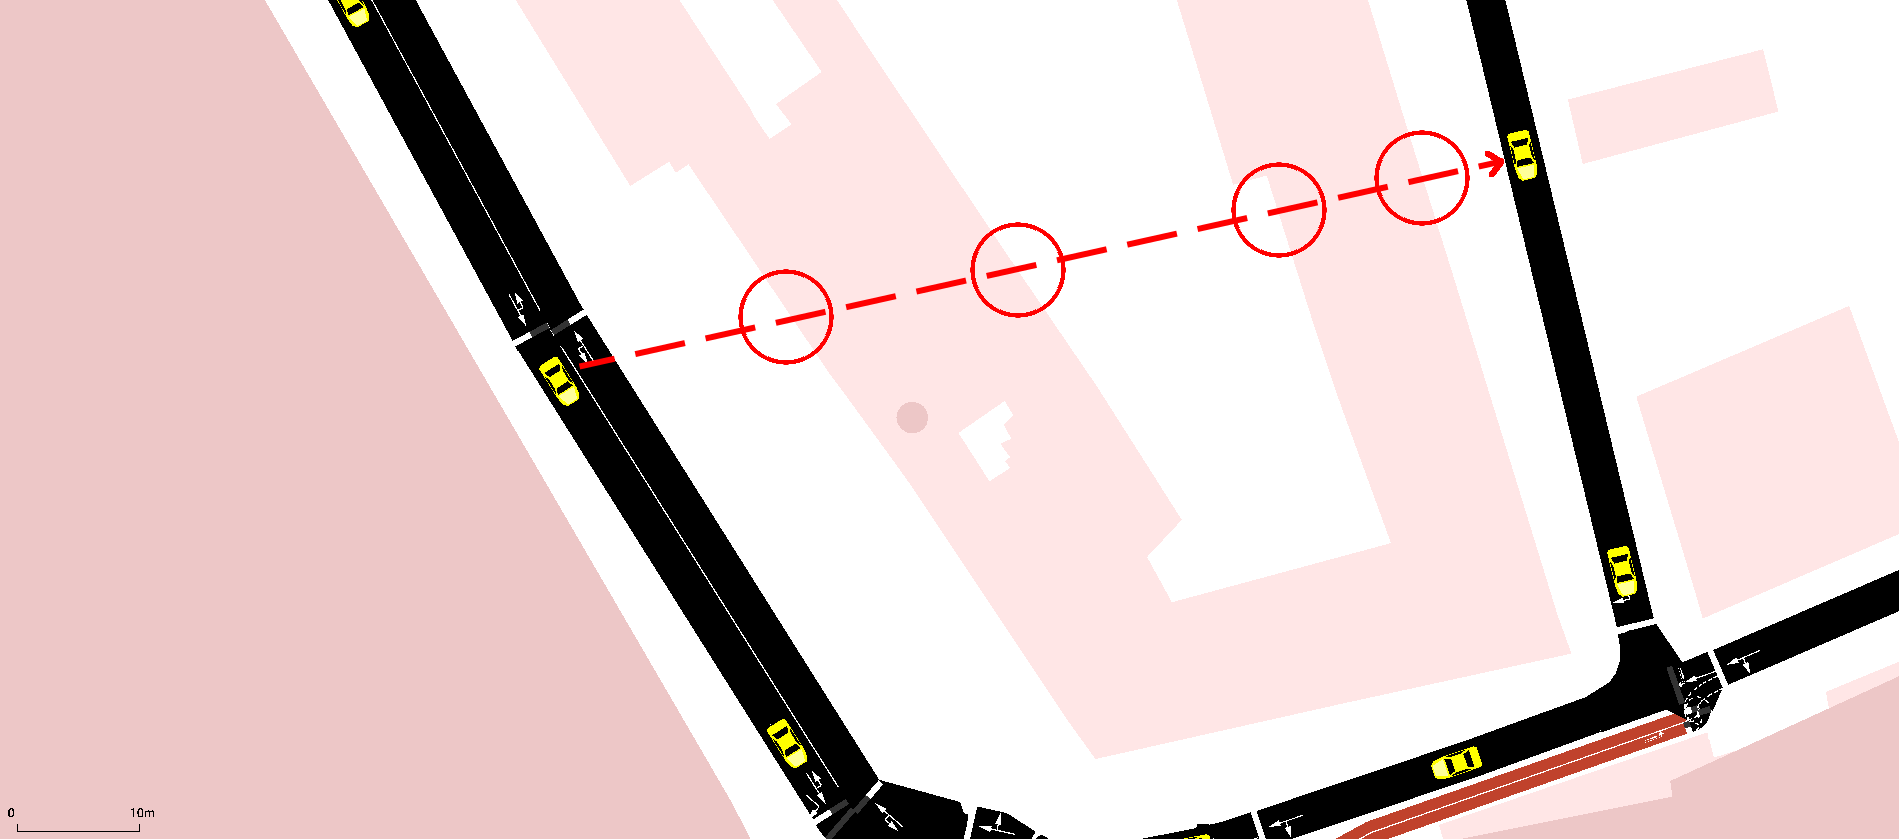
\includegraphics[width=\textwidth]{immagini/sumo-obstacle}
			\caption{Example of obstacle shadowing in vehicle-to-vehicle communication. Walls encountered by the signal are surrounded in red circles}
			\label{fig:sumo-obstacle}
		\end{figure}
	
	\section{Emergency Message Dissemination and broadcasting protocols}
		Emergency Message Dissemination (EMD) is a fundamental application in \acrshort{vaneta} to prevent traffic accidents, thereby reducing death and injury rates. Such task can be execute by the VANET itself by turning it into an infrastructure-less self-organizing network, where the dissemination is carried out by specific protocols. 
		
		
		Since the traffic information, especially the emergency data, has a broadcast-oriented nature (i.e. it is of public interest), it is more appropriate to disseminate it using broadcasting routing scheme rather than unicast or multicast ones. \cite{5989903}
%		suddivisione broadcasting protocols
		
		This choice leads to some advantages, such as:
		\begin{itemize}
			\item the fact that vehicles do not need to know the destination address and how to calculate a route towards it;
			\item a greater coverage of vehicles interested in the information, useful also in lossy scenarios, especially when paired with controlled redundancy schemes;
			\item a greater efficiency in bandwidth usage.
		\end{itemize}
		
		Advancements in research on this topic has lead to the development of a number of broadcasting protocols. However, as identified by   Panichpapiboon et al.\cite{5989903}, most of them belong to one of two main categories:
		\begin{itemize}
			\item Multi-hop Broadcasting Protocols, in which packets are transmitted through the network via flooding by some of the neighbors of the source. It is of utmost importance to reduce the number of redundant transmission in order not to waste bandwidth.
			\item Single-hop Broadcasting Protocols, in which no flooding is employed. Instead, vehicles periodically select and broadcast only a subset of the packets it has received.
		\end{itemize}
		
		Multi-hop Broadcasting Protocols can be further subdivided into three categories:
		\begin{enumerate}
			\item Delay based protocols, which assign a different waiting time before rebroadcasting the message to each vehicle. This delay is usually inversely proportional to the distance between the source and the potential sender.
			Some examples are:
			\begin{itemize}
				\renewcommand\labelitemi{--}
				\item \textit{Urban Multi-hop Broadcast (UMB)} \cite{Korkmaz:2004:UMB:1023875.1023887}, designed to solve the broadcast redundancy, hidden node and reliability problems in multi-hop broadcasting using \textit{Request-to-Broadcast (RTB)} and \textit{Clear-To-Broadcast (CTB)} packets; 
				\item \textit{Smart Broadcast (SB)} \cite{4025102} and \textit{Efficient Directional Broadcast (EDB)} \cite{4340158}, which try to reduce the delay introduced by UMB and remove the RTB and CTB packets, respectively;
				\item \textit{Vehicle-density-based Emergency Broadcasting (VDEB)} \cite{5663803}, a slotted broadcasting protocol which keeps vehicle density into consideration when computing waiting time slots;
				\item \textit{Reliable Method for Disseminating Safety Information
				(RMDSI)} \cite{4591259}, which aims to offer better performances when the network becomes fragmented by making a forwarder keep a copy of the packet it has broadcasted until it hears a retransmission (or until the packet lifetime expires). If no retransmission is heard within a certain time limit, the forwarder tries to find the next node which can relay the message using a small control packet;
				\item \textit{Multi-hop Vehicular Broadcast (MHVB)} \cite{4068699}, a protocol that keeps traffic congestion into consideration by   checking whether the number of neighbors of a vehicle is greather than a certain threshold and its speed is less than another threshold. When a node detects congestion, it increases its broadcast interval in order to try to reduce the network load;
				\item \textit{Reliable Broadcasting of Life Safety Messages (RBLSM)} \cite{4458046}, whose main objective is reliability, and a higher priority is given to the vehicle nearest to the sender instead to the one furthest from it, due to the assumption that the closer the vehicle is, the more reliable it is considered since its received signal strength is higher.
			\end{itemize}
		
			\item Probabilistic-based Multi-hop Broadcasting Protocols
			The idea behind these kind of protocols is similar to the one behind Delay based protocols, but instead of assigning a different rebroadcast delay to each vehicle, a different rebroadcast probability is assigned. Each protocol differs in the function that assigns probabilities. Some examples of probabilistic-based protocols are:
			\begin{itemize}
				\renewcommand\labelitemi{--}
		 		\item \textit{Weighted p-Persistence} \cite{4407231}, in which every PFC computes its own rebroadcast probability based on distance between itself and the transmitter. The formula used is the following:
				\begin{gather}
		 			p_{ij} = \frac{D_{ij}}{R}
		 			\label{eq:weighted-p-persistence}
 				\end{gather}
 				where $D_{ij}$ is the distance between transmitter \textit{i} and PFC \textit{j} and R is the transmission range. Given this function, the probability to rebroadcast is proportional to the distance between the PFC and the transmitter. The abovementioned formula does not keep into account vehicle density and also assumes that the transmission range is fixed and known to all vehicles.
 				
 				\item \textit{Optimized Adaptive Probabilistic Broadcast (OAPB)\cite{1543865} and AutoCast (AC) \cite{4350058}}, which both keep the vehicle density into consideration when computing the forwarding probability by making vehicle periodically exchange Hello messages. Thanks to those messages, each vehicle can compute the number of neighbors and then use this information accordingly.
 				
 				\item \textit{Irresponsible Forwarding (IF)} \cite{4740277}\cite{5426212}, a protocol that considers vehicle density like OAPB and AC, but the formula used is not a simple linear function. In fact, the rebroadcast probability assignment function is the following:
 				\begin{gather}
 					p = e^{-\frac{\rho_s(z-d)}{c}}
 				\end{gather}
 				where $\rho_s$ is the vehicle density, $z$ is the transmission range, $d$ is the distance between the PFC and the transmitter and $c\geq1$ is a shaping parameter which influences rebroadcast probability. Irresponsible Forwarding aims to offer a solution that can scale with network density.
 				
 				
			\end{itemize}
		\end{enumerate}